\documentclass[11pt,letterpaper,oneside]{report}

% -----------------------------------------------------------------------------
% Configuración general compatible con Overleaf (pdfLaTeX)
% -----------------------------------------------------------------------------
\usepackage[utf8]{inputenc}
\usepackage[T1]{fontenc}
\usepackage[spanish,es-nodecimaldot]{babel}
\usepackage{lmodern}
\usepackage{microtype}
\usepackage[letterpaper,margin=2.5cm,headheight=15pt]{geometry}
\usepackage{xcolor}
\usepackage{graphicx}
\usepackage{booktabs}
\usepackage{longtable}
\usepackage{tabularx}
\usepackage{array}
\usepackage{enumitem}
\usepackage{fancyhdr}
\usepackage{titlesec}
\usepackage{hyperref}
\usepackage{xurl}
\usepackage{amsmath}
\usepackage{amssymb}
\usepackage{siunitx}
\usepackage{caption}
\usepackage{float}
\usepackage{tikz}
\usetikzlibrary{arrows.meta,positioning,shapes.geometric}
\usepackage[most]{tcolorbox}
\usepackage{listings}
\usepackage{lastpage}

% -----------------------------------------------------------------------------
% Variables editables por el equipo
% -----------------------------------------------------------------------------
\newcommand{\ProjectTitle}{Observatorio territorial de hurto y reporte ciudadano en Bogotá}
\newcommand{\ProjectSubtitle}{Integración reproducible de delitos registrados, incidentes 123 y población por localidad}
\newcommand{\TeamName}{[Nombre del equipo]}
\newcommand{\TeamMembers}{[Integrante 1] \\ [Integrante 2] \\ [Integrante 3]}
\newcommand{\TeamEntity}{[Entidad u organización]}
\newcommand{\ContactEmail}{[Correo del líder del equipo]}
\newcommand{\ReportVersion}{0.3 -- Serie anual 2018--2025 validada}
\newcommand{\ReportDate}{1 de julio de 2026}

% -----------------------------------------------------------------------------
% Sistema visual institucional sobrio
% -----------------------------------------------------------------------------
\definecolor{GovNavy}{HTML}{14213D}
\definecolor{GovBlue}{HTML}{1F6E8C}
\definecolor{GovTeal}{HTML}{2A9D8F}
\definecolor{GovYellow}{HTML}{F4D35E}
\definecolor{GovLight}{HTML}{F5F7FA}
\definecolor{GovGray}{HTML}{5B6573}
\definecolor{GovRed}{HTML}{B23A48}

\hypersetup{
  colorlinks=true,
  linkcolor=GovNavy,
  citecolor=GovBlue,
  urlcolor=GovBlue,
  pdftitle={\ProjectTitle},
  pdfauthor={\TeamName},
  pdfsubject={Bogotá DataJam - Edición 2 - 2026},
  pdfkeywords={datos abiertos, seguridad, Bogotá, reproducibilidad, hurto, localidades}
}

\pagestyle{fancy}
\fancyhf{}
\fancyhead[L]{\small\textcolor{GovGray}{Bogotá DataJam -- Edición 2}}
\fancyhead[R]{\small\textcolor{GovGray}{\TeamName}}
\fancyfoot[L]{\small\textcolor{GovGray}{\ReportVersion}}
\fancyfoot[R]{\small\textcolor{GovGray}{Página \thepage\ de \pageref{LastPage}}}
\renewcommand{\headrulewidth}{0.4pt}
\renewcommand{\footrulewidth}{0.4pt}

\titleformat{\chapter}[display]
  {\normalfont\bfseries\color{GovNavy}}
  {\filleft\Large\chaptertitlename\ \thechapter}
  {0.5ex}
  {\titlerule\vspace{1ex}\Huge}
\titleformat{\section}{\Large\bfseries\color{GovBlue}}{\thesection}{0.75em}{}
\titleformat{\subsection}{\large\bfseries\color{GovNavy}}{\thesubsection}{0.75em}{}

\setlist[itemize]{leftmargin=1.5em,itemsep=0.35em,topsep=0.35em}
\setlist[enumerate]{leftmargin=1.7em,itemsep=0.35em,topsep=0.35em}
\renewcommand{\arraystretch}{1.2}
\sisetup{group-separator={.},group-minimum-digits=4,output-decimal-marker={,}}

\newcolumntype{Y}{>{\raggedright\arraybackslash}X}
\newcolumntype{C}[1]{>{\centering\arraybackslash}p{#1}}
\newcolumntype{L}[1]{>{\raggedright\arraybackslash}p{#1}}

\newtcolorbox{keybox}[1]{
  colback=GovLight,
  colframe=GovBlue,
  title=\textbf{#1},
  fonttitle=\color{white},
  arc=2mm,
  boxrule=0.8pt
}

\newtcolorbox{warningbox}[1]{
  colback=GovYellow!18,
  colframe=GovYellow!70!black,
  title=\textbf{#1},
  fonttitle=\color{black},
  arc=2mm,
  boxrule=0.8pt
}

\newtcolorbox{pendingbox}{
  colback=GovYellow!15,
  colframe=GovYellow!70!black,
  title=\textbf{Sección pendiente de actualización},
  fonttitle=\color{black},
  arc=2mm,
  boxrule=0.8pt
}

\lstdefinestyle{reproducible}{
  basicstyle=\ttfamily\small,
  backgroundcolor=\color{GovLight},
  frame=single,
  rulecolor=\color{GovBlue!45},
  breaklines=true,
  showstringspaces=false,
  columns=fullflexible,
  keepspaces=true
}

\begin{document}

% -----------------------------------------------------------------------------
% Portada
% -----------------------------------------------------------------------------
\begin{titlepage}
  \pagecolor{GovNavy}
  \color{white}
  \centering
  \vspace*{1.2cm}

  {\Large\bfseries Bogotá DataJam: Uso y Aprovechamiento de Datos\par}
  \vspace{0.25cm}
  {\large Edición 2 -- 2026\par}

  \vfill

  \begin{tcolorbox}[
    width=0.92\textwidth,
    colback=white,
    colframe=GovYellow,
    boxrule=1.4pt,
    arc=3mm,
    left=8mm,right=8mm,top=8mm,bottom=8mm
  ]
    \centering
    {\Huge\bfseries\color{GovNavy}\ProjectTitle\par}
    \vspace{0.5cm}
    {\Large\color{GovBlue}\ProjectSubtitle\par}
  \end{tcolorbox}

  \vfill

  \begin{tabular}{rl}
    \textbf{Equipo:} & \TeamName \\
    \textbf{Integrantes:} & \begin{tabular}[t]{l}\TeamMembers\end{tabular} \\
    \textbf{Entidad:} & \TeamEntity \\
    \textbf{Contacto:} & \ContactEmail \\
    \textbf{Versión:} & \ReportVersion \\
    \textbf{Fecha:} & \ReportDate
  \end{tabular}

  \vfill
  {\small Bogotá D.C., Colombia\par}
\end{titlepage}
\nopagecolor

% -----------------------------------------------------------------------------
% Control documental
% -----------------------------------------------------------------------------
\pagenumbering{roman}

\chapter*{Control documental}
\addcontentsline{toc}{chapter}{Control documental}

\begin{tabularx}{\textwidth}{L{0.23\textwidth}Y}
\toprule
\textbf{Campo} & \textbf{Valor} \\
\midrule
Título & \ProjectTitle \\
Versión & \ReportVersion \\
Estado & Borrador técnico reproducible; análisis validado y dashboard en desarrollo \\
Responsable & \TeamName \\
Repositorio & [URL pública de GitHub o GitLab] \\
Dashboard & [URL pública del dashboard] \\
Licencia del código & [Definir licencia] \\
Fuentes & Portal de Datos Abiertos Bogotá \\
\bottomrule
\end{tabularx}

\section*{Historial de versiones}

\begin{tabularx}{\textwidth}{L{0.12\textwidth}L{0.18\textwidth}Y}
\toprule
\textbf{Versión} & \textbf{Fecha} & \textbf{Cambio} \\
\midrule
0.1 & 28 de junio de 2026 & Formulación, fuentes, auditoría de limpieza, integración, reproducibilidad, arquitectura y glosario. \\
0.2 & 28 de junio de 2026 & Validación temporal, análisis 2025--2026, hallazgos, visualizaciones y recomendaciones. \\
0.3 & 29 de junio de 2026 & Reconstrucción con fuentes anuales 2018--2025, control de cobertura territorial, nuevo Excel y visualizaciones. \\
\bottomrule
\end{tabularx}

\clearpage
\tableofcontents
\clearpage
\listoftables
\clearpage
\listoffigures
\clearpage

\pagenumbering{arabic}

% -----------------------------------------------------------------------------
\chapter{Resumen ejecutivo}

Este proyecto construye un observatorio territorial para comparar el hurto a personas entre las localidades de Bogotá mediante tres perspectivas diferenciadas: delitos registrados, incidentes ciudadanos comunicados al sistema 123 y población residente. El propósito es superar las comparaciones basadas únicamente en conteos absolutos, producir tasas territorialmente comparables y explorar brechas entre registro institucional y demanda de atención.

La solución integra los conjuntos públicos \textit{Delito de Alto Impacto}, \textit{Incidente Reportado} y \textit{Población en Bogotá D.C. 2005--2035}. Los archivos fueron auditados y transformados mediante scripts reproducibles. Los originales se preservaron sin modificación; no se eliminaron duplicados, vacíos ni valores atípicos porque la auditoría no encontró evidencia suficiente para descartarlos. Los registros sin geometría fueron separados de las capas cartográficas, pero se conservaron para mantener la trazabilidad.

El producto final será un dashboard cartográfico que permitirá comparar conteos, tasas por cada \num{100000} habitantes, variaciones y la relación entre incidentes 123 y hurtos registrados. Como componente experimental se plantea una capa de reportes comunitarios recibidos mediante WhatsApp o formulario web, claramente separada de las estadísticas oficiales y sometida a consentimiento, moderación y agregación espacial.

La serie anual completa cubre 2018--2025. Los hurtos a personas alcanzaron un máximo de \num{158747} en 2023, descendieron a \num{130504} en 2024 (\(-17{,}8\,\%\)) y a \num{123800} en 2025 (\(-5{,}1\,\%\)). En 2025 los incidentes 123 asociados a hurto aumentaron \(3{,}1\,\%\), por lo que las dos fuentes volvieron a evolucionar de manera distinta. El principal hallazgo de calidad es territorial: \num{21906} hurtos de 2025 quedaron sin localidad, equivalentes al \(17{,}7\,\%\) del total. Por ello el total distrital es utilizable, pero el mapa debe mostrar una advertencia y usar 2024 como vista territorial inicial.

\begin{keybox}{Aporte principal}
El MVP no pretende estimar la totalidad de delitos ocurridos ni demostrar causalidad. Su aporte consiste en organizar evidencia pública comparable, hacer visibles diferencias territoriales y documentar las brechas y limitaciones que deben considerar las entidades al priorizar análisis o intervenciones.
\end{keybox}

% -----------------------------------------------------------------------------
\chapter{Trazabilidad frente a los requisitos del DataJam}

\begin{longtable}{L{0.29\textwidth}L{0.43\textwidth}C{0.15\textwidth}}
\caption{Matriz de cumplimiento de entregables y criterios}\label{tab:compliance}\\
\toprule
\textbf{Requisito} & \textbf{Evidencia en este proyecto} & \textbf{Estado} \\
\midrule
\endfirsthead
\toprule
\textbf{Requisito} & \textbf{Evidencia en este proyecto} & \textbf{Estado} \\
\midrule
\endhead
Problema público, pregunta e hipótesis & Capítulo \ref{chap:formulacion} & Completo \\
Mínimo dos fuentes públicas & Tres fuentes públicas descritas en el capítulo \ref{chap:datos} & Completo \\
Limpieza, transformación e integración & Capítulos \ref{chap:metodologia} y \ref{chap:auditoria} & Completo \\
Análisis reproducible & Scripts, estructura y comandos del capítulo \ref{chap:reproducibilidad} & Completo \\
Visualización o dashboard & Diseño funcional del capítulo \ref{chap:dashboard} & En desarrollo \\
Formulario de caracterización & Información base consolidada en este documento & Por diligenciar \\
Nota técnica de integración & Síntesis del capítulo \ref{chap:integracion} & Completo \\
Resultados y recomendaciones & Capítulos \ref{chap:resultados} y \ref{chap:recomendaciones} & Completo \\
Pitch final & Estructura narrativa derivada del resumen ejecutivo & Pendiente \\
\bottomrule
\end{longtable}

% -----------------------------------------------------------------------------
\chapter{Formulación del problema}\label{chap:formulacion}

\section{Problema público}

Los conteos de hurtos registrados no permiten comparar directamente las localidades de Bogotá, pues estas difieren ampliamente en tamaño poblacional y dinámica territorial. Además, la relación entre delitos registrados e incidentes ciudadanos asociados a hurto puede variar entre localidades. Sin una integración explícita de estas fuentes, la lectura territorial puede sobrerrepresentar localidades grandes, ocultar concentraciones relativas y conducir a interpretaciones incompletas para la toma de decisiones.

\section{Justificación}

La seguridad ciudadana es un asunto público que afecta el uso del espacio, la movilidad, la actividad económica y la confianza institucional. Un análisis reproducible y territorialmente comparable permite identificar patrones que requieren profundización, orientar preguntas de política pública y comunicar las limitaciones de los registros administrativos. La escala de localidad también facilita vincular los resultados con capacidades institucionales y decisiones de gestión local.

\section{Delimitación}

\begin{itemize}
  \item \textbf{Territorial:} veinte localidades de Bogotá D.C. Los registros sin localización se conservan, pero no se representan en el mapa.
  \item \textbf{Temporal:} años completos enero--diciembre de 2018 a 2025. El acumulado enero--mayo de 2026 se conserva en una tabla separada y no se mezcla con la serie anual.
  \item \textbf{Temática:} hurto a personas como indicador principal; otras categorías de alto impacto se conservan para exploraciones posteriores.
  \item \textbf{Poblacional:} población residente proyectada por localidad y año.
  \item \textbf{Analítica:} alcance descriptivo y exploratorio. No se realizarán afirmaciones causales.
\end{itemize}

\section{Pregunta de análisis}

\begin{keybox}{Pregunta principal}
¿Cómo evolucionaron anualmente los hurtos a personas en Bogotá entre 2018 y 2025, qué diferencias existen entre conteos y tasas por localidad y cómo se relacionan con los incidentes de hurto comunicados al 123?
\end{keybox}

\section{Hipótesis preliminar}

Las localidades con más hurtos en valores absolutos no serán necesariamente las de mayor tasa por cada \num{100000} habitantes. Asimismo, existirán localidades donde la relación entre incidentes 123 y delitos registrados sea atípicamente alta o baja, lo cual puede señalar diferencias territoriales en reporte, demanda de atención o registro que requieren análisis adicional.

Esta hipótesis es exploratoria. Una asociación entre fuentes no equivale a causalidad ni permite estimar directamente el subregistro delictivo.

\section{Objetivos}

\subsection{Objetivo general}

Construir un análisis territorial reproducible del hurto a personas en Bogotá que integre delitos registrados, incidentes 123 y población por localidad, con el fin de producir indicadores comparables y apoyar la interpretación de diferencias territoriales.

\subsection{Objetivos específicos}

\begin{enumerate}
  \item Auditar, limpiar y estandarizar las fuentes públicas seleccionadas sin alterar los archivos originales.
  \item Integrar las fuentes mediante código de localidad y año, documentando granularidad, cobertura y limitaciones.
  \item Calcular conteos anuales, tasas por cada \num{100000} habitantes, variaciones interanuales y medidas exploratorias de brecha de reporte.
  \item Desarrollar un dashboard cartográfico que facilite la comparación entre localidades, indicadores y años completos de 2018 a 2025.
  \item Diseñar una capa comunitaria separada de las cifras oficiales, con controles de privacidad, moderación y calidad.
\end{enumerate}

% -----------------------------------------------------------------------------
\chapter{Fuentes de datos}\label{chap:datos}

\begin{table}[H]
\centering
\caption{Fuentes principales del análisis}\label{tab:sources}
\begin{tabularx}{\textwidth}{L{0.22\textwidth}L{0.18\textwidth}L{0.2\textwidth}Y}
\toprule
\textbf{Fuente} & \textbf{Entidad} & \textbf{Granularidad usada} & \textbf{Función analítica} \\
\midrule
Delito de Alto Impacto & Secretaría Distrital de Seguridad, Convivencia y Justicia & Localidad y año completo & Numerador de hurtos a personas registrados. \\
Incidente Reportado & Secretaría Distrital de Seguridad, Convivencia y Justicia & Localidad y año completo & Demanda ciudadana de atención asociada a hurto. \\
Población en Bogotá D.C. 2005--2035 & Secretaría Distrital de Salud & Localidad, año, sexo y edad & Denominador para tasas territoriales. \\
\bottomrule
\end{tabularx}
\end{table}

\section{Campos utilizados}

\begin{itemize}
  \item \textbf{Seguridad:} código y nombre de localidad, etiqueta de periodo, conteos anuales por categoría y geometría territorial.
  \item \textbf{Población:} año, código y nombre de localidad, sexo, edad, curso de vida, grupo etario y población.
  \item \textbf{Integración:} código de localidad normalizado a dos caracteres y año.
\end{itemize}

\section{Distinción conceptual entre fuentes}

Un \textbf{delito registrado} es un hecho incluido en un sistema administrativo; un \textbf{incidente 123} corresponde a una llamada ciudadana trasladada a una agencia de respuesta; y un \textbf{reporte comunitario} es información autodeclarada en el canal experimental del proyecto. Los tres conceptos miden fenómenos relacionados, pero no intercambiables.

% -----------------------------------------------------------------------------
\chapter{Metodología}\label{chap:metodologia}

\section{Ruta metodológica D.A.T.O.S.}

La metodología se organizó siguiendo la ruta presentada en el DataJam:

\begin{enumerate}[label=\textbf{\Alph*.}]
  \item \textbf{Definir:} delimitación del problema público, población, territorio y periodo.
  \item \textbf{Aterrizar:} definición de unidad de análisis, variables e indicadores.
  \item \textbf{Trabajar/testear:} auditoría de disponibilidad, calidad, granularidad y llaves de integración.
  \item \textbf{Observar:} documentación de sesgos, vacíos, incompatibilidades y riesgos de interpretación.
  \item \textbf{Sintetizar:} producción de hallazgos interpretables, visualizaciones y recomendaciones aplicables.
\end{enumerate}

\section{Flujo reproducible}

\begin{figure}[H]
\centering
\begin{tikzpicture}[
  node distance=7mm and 6mm,
  box/.style={rectangle,rounded corners=2mm,draw=GovBlue,fill=GovLight,minimum height=11mm,text width=3.0cm,align=center,font=\small},
  arrow/.style={-{Latex[length=2.5mm]},thick,color=GovTeal}
]
\node[box] (raw) {Archivos originales\\\texttt{data/raw}};
\node[box,right=of raw] (profile) {Perfilamiento\\esquema y calidad};
\node[box,right=of profile] (clean) {Limpieza y\\normalización};
\node[box,below=of clean] (integrate) {Integración y\\cálculo de tasas};
\node[box,left=of integrate] (validate) {Validaciones\\automáticas};
\node[box,left=of validate] (publish) {Datos procesados\\y dashboard};
\draw[arrow] (raw) -- (profile);
\draw[arrow] (profile) -- (clean);
\draw[arrow] (clean) -- (integrate);
\draw[arrow] (integrate) -- (validate);
\draw[arrow] (validate) -- (publish);
\end{tikzpicture}
\caption{Flujo de preparación e integración de datos}
\label{fig:pipeline}
\end{figure}

\section{Reglas de limpieza}

\begin{enumerate}
  \item Preservar los originales y registrar su huella SHA-256.
  \item Eliminar únicamente duplicados exactos verificables.
  \item No imputar conteos ni población sin una regla metodológica justificable.
  \item Separar los registros sin geometría de las salidas cartográficas, conservándolos en archivos tabulares.
  \item Normalizar códigos, nombres y tipos de datos antes de integrar.
  \item Marcar valores atípicos para revisión, sin eliminarlos automáticamente.
  \item Mantener explícita la etiqueta temporal del archivo para evitar comparaciones entre periodos incompatibles.
\end{enumerate}

% -----------------------------------------------------------------------------
\chapter{Auditoría y limpieza}\label{chap:auditoria}

\section{Inventario y preservación}

Se procesaron cinco archivos: un CSV poblacional y cuatro GeoJSON. Las copias almacenadas en \texttt{data/raw/} coinciden byte a byte con los archivos entregados, según SHA-256. Ningún proceso escribe sobre los originales.

\section{Resultados de calidad}

\begin{table}[H]
\centering
\caption{Resumen de decisiones de limpieza}\label{tab:cleaning}
\begin{tabularx}{\textwidth}{Y C{0.18\textwidth} Y}
\toprule
\textbf{Control} & \textbf{Resultado} & \textbf{Decisión} \\
\midrule
Duplicados exactos & 0 & No se eliminaron registros. \\
Filas vacías en población & 0 & No se eliminaron registros. \\
Métricas faltantes usadas & 0 & No se aplicó imputación. \\
Outliers eliminados & 0 & Los extremos se conservaron. \\
Valores marcados por IQR en el análisis anual & 29 & Revisión analítica, sin eliminación. \\
Filas de población con valor cero & 526 & Se conservaron; corresponden a celdas demográficas específicas. \\
Geometrías nulas en localidad & 2 & Se separaron los códigos 99 de las capas de mapa. \\
Geometría nula en UPZ & 1 & Se separó \texttt{UPZ999}. \\
\bottomrule
\end{tabularx}
\end{table}

\section{Población}

El archivo de población contiene \num{131502} filas. Se separaron \num{6262} filas correspondientes al agregado \texttt{00 -- Bogotá}, evitando doble conteo al sumar las veinte localidades. Las \num{125240} filas restantes se conservaron como detalle por localidad, sexo, edad y año. La agregación anual produjo 620 filas: veinte localidades por 31 años. La diferencia entre el agregado distrital de la fuente y la suma de las localidades fue cero para todos los años.

\section{Delito de Alto Impacto}

La capa anual contenía 21 elementos: veinte localidades con geometría y un registro \texttt{99 -- Sin Localización} sin geometría. El mapa limpio conserva las veinte localidades. Las métricas se normalizaron a \num{1848} filas: 21 unidades, once categorías y ocho años completos. En 2025 se identificaron \num{21906} hurtos a personas sin localidad, equivalentes al \(17{,}7\,\%\) del total anual; se conservaron en los totales distritales y se excluyeron únicamente de la cartografía.

\section{Incidentes reportados}

La capa anual de localidad contenía 21 elementos: veinte localidades cartografiables y un registro \texttt{Sin Localización}. Se produjeron \num{1512} observaciones en estructura larga: 21 unidades, nueve categorías y ocho años completos. Para el cruce principal se utilizó la categoría general de incidente por hurto.

\section{Normalizaciones aplicadas}

\begin{itemize}
  \item Códigos de localidad con longitud fija de dos caracteres.
  \item Nombre \textit{Candelaria} normalizado a \textit{La Candelaria} según el catálogo poblacional.
  \item Conversión explícita de año, edad, población y conteos a tipos numéricos.
  \item Transformación de columnas anchas por año a estructura larga.
  \item Creación de una única geometría base de localidades, pues las dos fuentes de seguridad coincidieron en sus veinte geometrías.
\end{itemize}

\begin{warningbox}{Decisión sobre valores atípicos}
El método IQR 1,5 marcó 29 valores en la tabla anual: 21 conteos altos de incidentes 123, seis tasas altas de hurto y dos tasas altas de incidentes. No se eliminaron: un valor extremo puede reflejar tamaño poblacional, centralidad, población flotante o una dinámica auténtica. El tratamiento correcto es revisarlo y documentarlo, no borrarlo mecánicamente.
\end{warningbox}

% -----------------------------------------------------------------------------
\chapter{Integración e indicadores}\label{chap:integracion}

\section{Llave de integración}

Las fuentes se integraron mediante \texttt{locality\_code + year}. El código se estandarizó a dos caracteres y los nombres se reconciliaron con el catálogo poblacional. La tabla anual resultante contiene 160 filas, correspondientes a veinte localidades y ocho años completos entre 2018 y 2025. No se encontraron filas sin emparejar, duplicados de llave ni poblaciones faltantes.

\section{Indicadores}

Sea $H_{l,t}$ el número anual de hurtos a personas registrados en la localidad $l$ durante el año completo $t$, $I_{l,t}$ los incidentes 123 asociados a hurto y $P_{l,t}$ la población residente proyectada.

\subsection{Tasa anual de hurto}

\begin{equation}
T^{H}_{l,t}=\frac{H_{l,t}}{P_{l,t}}\times 100\,000
\end{equation}

\subsection{Tasa anual de incidentes}

\begin{equation}
T^{I}_{l,t}=\frac{I_{l,t}}{P_{l,t}}\times 100\,000
\end{equation}

\subsection{Razón exploratoria de incidentes por hurto registrado}

\begin{equation}
R_{l,t}=\frac{I_{l,t}}{H_{l,t}}, \qquad H_{l,t}>0
\end{equation}

La razón no se calcula cuando $H_{l,t}=0$; en ese caso se conserva como nula en lugar de reemplazarse por cero o infinito.

\section{Nota técnica de integración}

La integración fue viable porque las tres fuentes comparten código de localidad y año. Se utilizaron los recursos oficiales separados de enero--diciembre para Delito de Alto Impacto e Incidente Reportado, ambos con cobertura 2018--2025. El dato enero--mayo de 2026 permanece separado. La principal dificultad analítica es semántica: un delito registrado y una llamada 123 representan procesos distintos; adicionalmente, la asignación territorial de hurtos se deteriora en 2025.

% -----------------------------------------------------------------------------
\chapter{Resultados analíticos}\label{chap:resultados}

\section{Alcance de la comparación}

Los resultados utilizan años completos enero--diciembre de 2018 a 2025. La referencia enero--mayo de 2026 se conserva fuera de la serie y no se utiliza para calcular variaciones anuales. Los totales distritales incluyen registros sin localización; las visualizaciones territoriales solo pueden representar los registros asignados a una de las veinte localidades.

\section{Hallazgo principal: la trayectoria anual presenta cambios de dirección}

Los hurtos a personas pasaron de \num{105943} en 2018 a \num{127828} en 2019; descendieron \(35{,}0\,\%\) en 2020 y luego aumentaron hasta un máximo de \num{158747} en 2023. Posteriormente disminuyeron a \num{130504} en 2024 (\(-17{,}8\,\%\)) y a \num{123800} en 2025 (\(-5{,}1\,\%\)). El nivel de 2025 continúa \(16{,}9\,\%\) por encima del observado en 2018.

Los incidentes 123 asociados a hurto siguieron otra trayectoria: en 2025 aumentaron de \num{134964} a \num{139082} (\(+3{,}1\,\%\)) mientras los hurtos registrados disminuyeron. Esta divergencia no demuestra subregistro ni permite afirmar que una fuente sea más correcta; muestra que denuncia o registro administrativo y demanda de atención no deben fusionarse como una sola medida.

\begin{figure}[H]
\centering
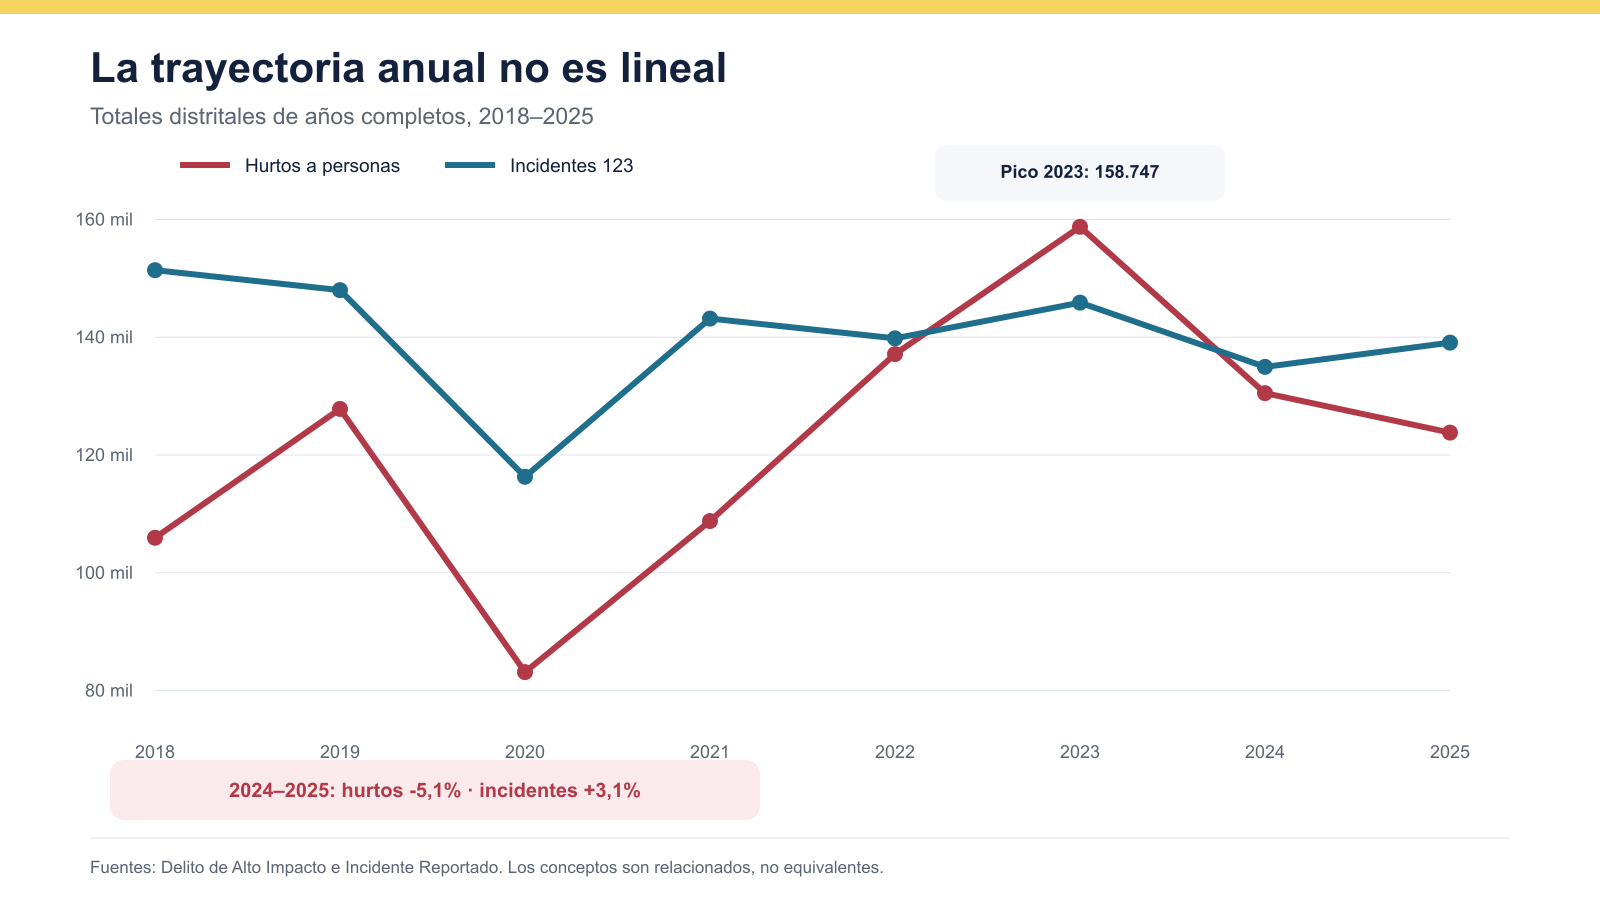
\includegraphics[width=\textwidth]{figures/fig_tendencia_anual_2018_2025.png}
\caption{Trayectoria distrital anual de hurtos a personas e incidentes 123, 2018--2025}
\label{fig:tendencia-anual}
\end{figure}

En 2025 la asociación territorial entre las dos fuentes fue alta (Pearson de 0,898 y Spearman de 0,869), por lo que describen patrones relacionados, pero no sustituibles.

\section{Hallazgo secundario 1: 2025 tiene una ruptura de cobertura territorial}

En 2025 se registraron \num{21906} hurtos a personas sin localidad asignada, equivalentes al \(17{,}7\,\%\) del total distrital. La cobertura cartografiable cayó a \(82{,}3\,\%\), mientras en 2024 fue \(99{,}4\,\%\). Esto significa que el total de Bogotá puede utilizarse, pero las comparaciones entre localidades de 2025 pueden estar sesgadas por pérdida diferencial de geocodificación.

Por esta razón, el dashboard debe utilizar 2024 como vista territorial inicial y permitir 2025 únicamente con una alerta visible de cobertura. No sería válido atribuir automáticamente a cada localidad las disminuciones observadas entre 2024 y 2025.

\begin{figure}[H]
\centering
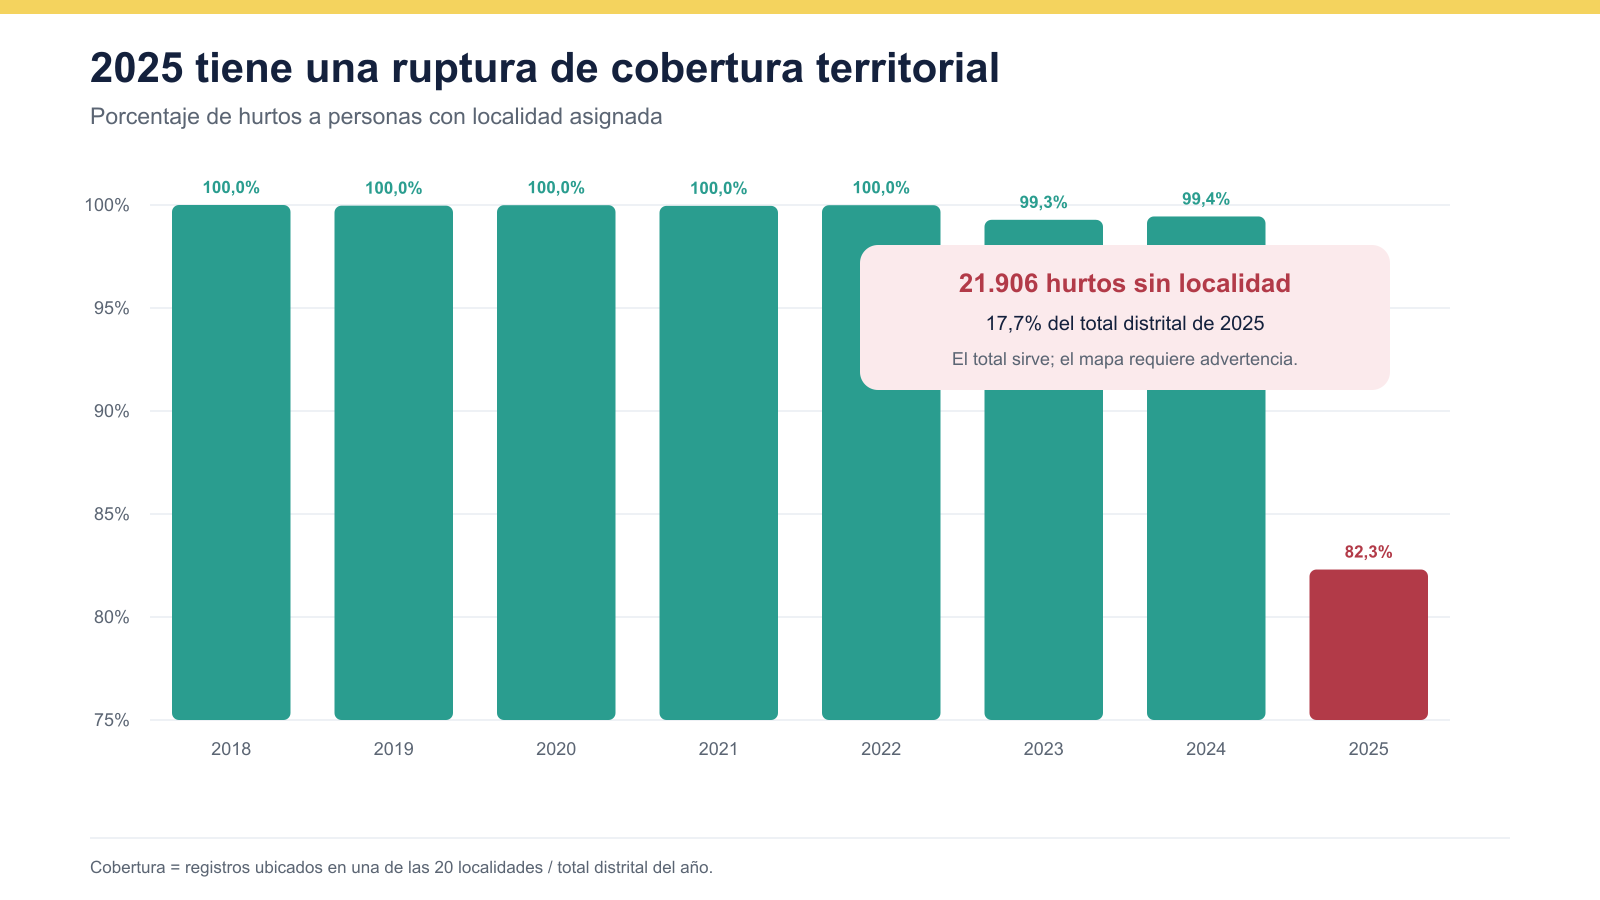
\includegraphics[width=\textwidth]{figures/fig_cobertura_territorial_anual.png}
\caption{Cobertura territorial anual de los registros de hurto a personas}
\label{fig:cobertura-territorial}
\end{figure}

\section{Hallazgo secundario 2: conteos y tasas producen mapas distintos}

Para evitar el sesgo territorial de 2025, se tomó 2024 como año de referencia espacial. Los mayores conteos se observaron en Suba (\num{12836}), Engativá (\num{12343}), Kennedy (\num{11961}), Los Mártires (\num{11499}) y Chapinero (\num{10977}). Las mayores tasas por cada \num{100000} habitantes correspondieron a Los Mártires (\num{15250.1}), La Candelaria (\num{10773.6}), Santa Fe (\num{8458.5}), Chapinero (\num{6788.7}) y Teusaquillo (\num{4867.3}).

La asociación de rangos entre conteo y tasa fue baja (Spearman de 0,296). Suba ocupó el primer puesto por conteo y el 14 por tasa; La Candelaria pasó del puesto 19 por conteo al segundo por tasa. Por tanto, el dashboard debe permitir alternar ambas medidas y explicar que la población residente no representa la población flotante de las localidades centrales.

\begin{figure}[H]
\centering
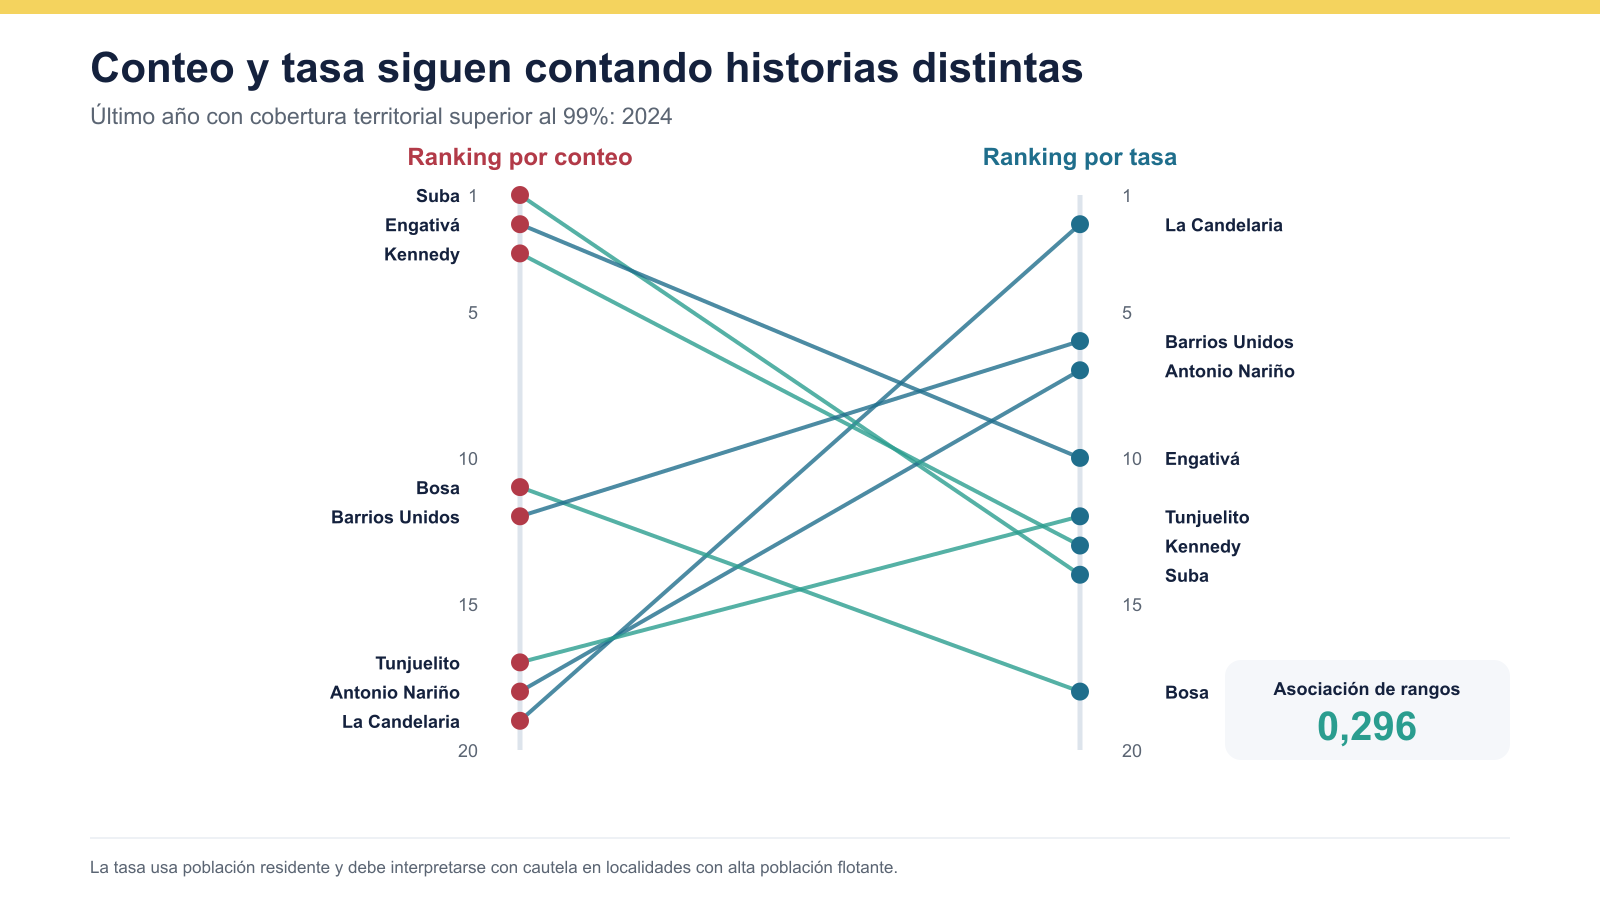
\includegraphics[width=\textwidth]{figures/fig_ranking_anual_2024.png}
\caption{Diferencias entre ranking por conteo y ranking por tasa en 2024}
\label{fig:ranking-anual-2024}
\end{figure}

\section{Revisión de valores atípicos}

En la serie anual se revisaron 29 marcas IQR: 21 conteos altos de incidentes 123, seis tasas altas de hurto y dos tasas altas de incidentes. Todos los valores se conservaron porque los extremos son coherentes con tamaño poblacional, centralidad o población flotante y no existe evidencia de error de captura. El crecimiento de registros sin localización en 2025 se trató como problema de cobertura, no como outlier eliminable.

\section{Evaluación de la hipótesis}

La hipótesis se respalda parcialmente: el ranking por conteo difiere del ranking por tasa y las fuentes presentan trayectorias distintas. No se respalda una interpretación causal ni una estimación directa de subregistro. El nuevo hallazgo de cobertura obliga además a separar conclusiones distritales y territoriales para 2025.

% -----------------------------------------------------------------------------
\chapter{Dashboard y componente comunitario}\label{chap:dashboard}

\section{Mapa principal}

El dashboard utilizará un mapa coroplético por localidad con 2024 como vista territorial inicial, por ser el año completo más reciente con cobertura superior al \(99\,\%\). Permitirá seleccionar años completos de 2018 a 2025, fuente e indicador: hurtos registrados, incidentes 123, conteo, tasa por cada \num{100000} habitantes, variación interanual o relación entre fuentes. La selección de 2025 activará una advertencia de cobertura territorial del \(82{,}3\,\%\). La referencia enero--mayo de 2026 se mostrará en una sección parcial separada.

El MVP deberá incluir cuatro tarjetas distritales, selector de año, selector conteo/tasa, leyenda explícita, indicador de cobertura cartografiable, ranking ordenable y panel emergente por localidad. La capa comunitaria se mostrará mediante un control independiente y nunca se sumará a las cifras oficiales.

\section{Capa comunitaria}

El reporte comunitario podrá recibirse mediante WhatsApp o formulario web. El flujo propuesto es:

\begin{enumerate}
  \item Advertencia: el canal no reemplaza una denuncia ni la línea 123.
  \item Consentimiento informado para uso estadístico.
  \item Tipo de evento: hurto consumado o intento.
  \item Fecha y hora aproximadas.
  \item Localidad y ubicación aproximada.
  \item Categoría del objeto, modalidad y arma observada.
  \item Descripción opcional, confirmación y código del reporte.
\end{enumerate}

No se solicitará el nombre. Los datos privados no se publicarán y los reportes solo aparecerán agregados después de moderación.

\begin{figure}[H]
\centering
\begin{tikzpicture}[
  node distance=7mm,
  box/.style={rectangle,rounded corners=2mm,draw=GovBlue,fill=GovLight,minimum height=10mm,text width=4.3cm,align=center,font=\small},
  arrow/.style={-{Latex[length=2.5mm]},thick,color=GovTeal}
]
\node[box] (channel) {WhatsApp o formulario web};
\node[box,below=of channel] (webhook) {Webhook y máquina de conversación};
\node[box,below=of webhook] (moderation) {Validación, privacidad y moderación};
\node[box,below=of moderation] (private) {Almacenamiento privado del MVP};
\node[box,below=of private] (api) {API sanitizada y agregada};
\node[box,below=of api] (dashboard) {Capa comunitaria del dashboard};
\draw[arrow] (channel) -- (webhook);
\draw[arrow] (webhook) -- (moderation);
\draw[arrow] (moderation) -- (private);
\draw[arrow] (private) -- (api);
\draw[arrow] (api) -- (dashboard);
\end{tikzpicture}
\caption{Arquitectura conceptual del reporte comunitario}
\label{fig:community}
\end{figure}

% -----------------------------------------------------------------------------
\chapter{Reproducibilidad}\label{chap:reproducibilidad}

\section{Estructura del repositorio}

\begin{lstlisting}[style=reproducible]
data/
  raw/                  # Copias inmutables de las fuentes
  processed/            # Datos limpios e integrados
docs/                   # Definición del MVP y documento técnico
reports/                # Perfil, auditoría, validaciones y outliers
scripts/                # Código reproducible de preparación
\end{lstlisting}

\section{Secuencia de ejecución}

\begin{lstlisting}[style=reproducible,language=bash]
python scripts/build_annual_pipeline.py .
node scripts/render_annual_charts.cjs
node .tmp_sheet_build/build_annual_workbook.mjs
\end{lstlisting}

\section{Controles automáticos}

\begin{itemize}
  \item Conteo esperado de 160 filas integradas.
  \item Veinte localidades y ocho años completos entre 2018 y 2025.
  \item Unicidad de localidad y año.
  \item Cobertura completa de población.
  \item Conteos no negativos.
  \item Etiquetas enero--diciembre compatibles en las dos fuentes de seguridad.
  \item Tasas sin valores nulos.
  \item Coincidencia de las geometrías de localidad entre fuentes.
\end{itemize}

% -----------------------------------------------------------------------------
\chapter{Ética, privacidad y uso responsable}

\section{Principios}

\begin{itemize}
  \item \textbf{Finalidad:} recolectar solo información necesaria para análisis territorial agregado.
  \item \textbf{Minimización:} no solicitar nombre ni publicar teléfono, dirección exacta o relato identificable.
  \item \textbf{Consentimiento:} informar el uso antes de registrar datos comunitarios.
  \item \textbf{Separación:} no presentar reportes comunitarios como denuncias o hechos confirmados.
  \item \textbf{Seguridad:} mantener credenciales y datos privados fuera del frontend.
  \item \textbf{Moderación:} revisar duplicados, spam, contenido sensible y ubicaciones antes de agregar.
\end{itemize}

El tratamiento deberá observar la Ley 1581 de 2012 y las políticas aplicables de protección de datos personales. La versión pública solo expondrá agregados estadísticos.

% -----------------------------------------------------------------------------
\chapter{Limitaciones}

\begin{enumerate}
  \item Los registros administrativos no representan necesariamente la totalidad de hechos ocurridos.
  \item Un incidente 123 expresa una solicitud de atención; no confirma un delito.
  \item Los reportes comunitarios presentan sesgo de autoselección y acceso digital.
  \item La población proyectada es una estimación y describe residentes, no población flotante.
  \item Las tasas de localidades con poca población residente pueden ser sensibles a pequeñas variaciones.
  \item La serie anual termina en 2025. El dato 2026 disponible corresponde a enero--mayo y no es comparable con años completos.
  \item En 2025, el \(17{,}7\,\%\) de los hurtos a personas no tiene localidad asignada; esto limita comparaciones territoriales aunque no invalida el total distrital.
  \item Las relaciones observadas son descriptivas y no prueban causalidad.
  \item Las geometrías fuente están declaradas en EPSG:4686; su uso web debe mantener trazabilidad del sistema de referencia.
\end{enumerate}

% -----------------------------------------------------------------------------
\chapter{Recomendaciones y conclusiones}\label{chap:recomendaciones}

\section{Recomendaciones para el MVP}

\begin{enumerate}
  \item \textbf{Mostrar siempre conteo y tasa.} El tablero debe permitir alternarlos y conservar visible el denominador; la baja concordancia de rangos demuestra que cada medida responde una pregunta diferente.
  \item \textbf{Diferenciar las fuentes.} Hurtos registrados e incidentes 123 deben usar nombres, colores y explicaciones distintas. La variación distrital divergente impide tratarlos como una única cifra de inseguridad.
  \item \textbf{Priorizar años completos.} La tendencia debe utilizar 2018--2025. El dato enero--mayo de 2026 debe permanecer claramente separado hasta completar el año o construir una serie homogénea de primeros cinco meses.
  \item \textbf{Hacer visible la cobertura.} El mapa debe iniciar en 2024 y mostrar una alerta cuando se seleccione 2025, pues \num{21906} hurtos no tienen localidad asignada.
  \item \textbf{Advertir sobre población flotante.} Las tasas de La Candelaria, Santa Fe, Los Mártires, Chapinero y Teusaquillo requieren una nota visible porque el denominador representa residentes y no exposición diurna o población flotante.
\end{enumerate}

\section{Recomendaciones institucionales}

Se recomienda a la Secretaría Distrital de Seguridad, Convivencia y Justicia revisar el crecimiento de registros sin localidad en 2025, publicar el porcentaje de geocodificación como indicador de calidad y mantener separados los recursos enero--mayo y enero--diciembre. Como seguimiento puede medirse la cobertura territorial anual y el número de registros sin localización. Para análisis posteriores conviene incorporar población flotante, movilidad o afluencia como denominadores complementarios, sin reemplazar la población residente.

\section{Conclusión}

El MVP aporta una lectura más responsable que un ranking único de inseguridad: distingue volumen, riesgo relativo y demanda de atención, y hace explícito qué puede y qué no puede concluirse. La oportunidad de valor está en convertir esas diferencias en preguntas territoriales verificables y en una interfaz sencilla para equipos técnicos y ciudadanía.

% -----------------------------------------------------------------------------
\appendix
\chapter{Glosario}

\begin{longtable}{L{0.25\textwidth}L{0.67\textwidth}}
\toprule
\textbf{Término} & \textbf{Definición utilizada en el proyecto} \\
\midrule
\endfirsthead
\toprule
\textbf{Término} & \textbf{Definición utilizada en el proyecto} \\
\midrule
\endhead
Capa comunitaria & Visualización agregada de reportes comunitarios moderados, separada de la capa oficial. \\
Capa oficial & Visualización construida exclusivamente con fuentes públicas institucionales. \\
Delito registrado & Hecho incluido en Delito de Alto Impacto. No equivale a la totalidad de delitos ocurridos. \\
Fecha de corte & Último periodo comparable incluido en un análisis; no es necesariamente la fecha de actualización del portal. \\
Hurto a personas & Categoría principal usada para comparar localidades y años. \\
Incidente 123 & Llamada ciudadana trasladada a una agencia de respuesta. No es una denuncia ni un delito confirmado. \\
Outlier & Valor estadísticamente extremo que requiere revisión. No se considera error de manera automática. \\
Periodo comparable & Año completo enero--diciembre utilizado de forma consistente entre 2018 y 2025. \\
Reporte comunitario & Relato voluntario recibido por el proyecto, sin validez como denuncia oficial. \\
Tasa de hurto & Hurtos registrados durante el año completo por cada \num{100000} habitantes residentes. \\
Cobertura territorial & Porcentaje de registros distritales asignados a una de las veinte localidades y, por tanto, representables en el mapa. \\
Brecha de reporte & Diferencia o razón exploratoria entre incidentes 123 y hurtos registrados para una localidad y año. No estima directamente la cifra oculta. \\
\bottomrule
\end{longtable}

\chapter{Diccionario de la tabla integrada}

\begin{longtable}{L{0.33\textwidth}L{0.59\textwidth}}
\toprule
\textbf{Campo} & \textbf{Descripción} \\
\midrule
\endfirsthead
\toprule
\textbf{Campo} & \textbf{Descripción} \\
\midrule
\endhead
\texttt{locality\_code} & Código de localidad normalizado a dos caracteres. \\
\texttt{locality\_name} & Nombre canónico de la localidad. \\
\texttt{year} & Año completo de referencia, 2018--2025. \\
\texttt{coverage} & Cobertura temporal de la observación; \texttt{full\_year} para la tabla anual. \\
\texttt{registered\_person\_thefts} & Hurtos a personas registrados durante el año completo. \\
\texttt{reported\_123\_theft\_incidents} & Incidentes 123 asociados a hurto durante el año completo. \\
\texttt{population} & Población residente proyectada. \\
\texttt{theft\_rate\_per\_100k} & Tasa anual de hurto por cada \num{100000} habitantes. \\
\texttt{incident\_rate\_per\_100k} & Tasa anual de incidentes por cada \num{100000} habitantes. \\
\texttt{theft\_yoy\_pct} & Variación porcentual interanual de hurtos a personas por localidad. \\
\texttt{incident\_yoy\_pct} & Variación porcentual interanual de incidentes 123 por localidad. \\
\texttt{incidents\_per\_registered\_theft} & Razón exploratoria entre incidentes y hurtos; nula cuando el denominador es cero. \\
\texttt{count\_rank} & Posición de la localidad por conteo en cada año. \\
\texttt{rate\_rank} & Posición de la localidad por tasa en cada año. \\
\bottomrule
\end{longtable}

\chapter{Referencias}

\begin{thebibliography}{99}

\bibitem{reglas}
Secretaría General de la Alcaldía Mayor de Bogotá. (2026). \textit{Reglas de participación: Bogotá DataJam, Uso y Aprovechamiento de Datos, Edición 2}.

\bibitem{guia}
Secretaría General de la Alcaldía Mayor de Bogotá. (2026). \textit{Guía de entrega de resultados: Bogotá DataJam, Edición 2}.

\bibitem{metodologia}
Pontificia Universidad Javeriana. (2026). \textit{Formulación y desarrollo de un problema público: del tema general a una pregunta analítica viable}.

\bibitem{altoimpacto}
Secretaría Distrital de Seguridad, Convivencia y Justicia. (2026). \textit{Delito de Alto Impacto. Bogotá D.C.} Portal de Datos Abiertos Bogotá.\\
\url{https://datosabiertos.bogota.gov.co/dataset/delito-de-alto-impacto-bogota-d-c}

\bibitem{incidentes}
Secretaría Distrital de Seguridad, Convivencia y Justicia. (2026). \textit{Incidente Reportado. Bogotá D.C.} Portal de Datos Abiertos Bogotá.\\
\url{https://datosabiertos.bogota.gov.co/dataset/incidente-reportado-bogota-d-c}

\bibitem{poblacion}
Secretaría Distrital de Salud. (2026). \textit{Población en Bogotá D.C. 2005--2035}. Portal de Datos Abiertos Bogotá.\\
\url{https://datosabiertos.bogota.gov.co/dataset/piramide-poblacional-bogota-d-c}

\bibitem{ley1581}
Congreso de Colombia. (2012). \textit{Ley Estatutaria 1581 de 2012: disposiciones generales para la protección de datos personales}.\\
\url{https://www1.funcionpublica.gov.co/eva/gestornormativo/norma.php?i=49981}

\end{thebibliography}

\end{document}
